% THIS IS SIGPROC-SP.TEX - VERSION 3.1
% WORKS WITH V3.2SP OF ACM_PROC_ARTICLE-SP.CLS
% APRIL 2009
%
% It is an example file showing how to use the 'acm_proc_article-sp.cls' V3.2SP
% LaTeX2e document class file for Conference Proceedings submissions.
% ----------------------------------------------------------------------------------------------------------------
% This .tex file (and associated .cls V3.2SP) *DOES NOT* produce:
%       1) The Permission Statement
%       2) The Conference (location) Info information
%       3) The Copyright Line with ACM data
%       4) Page numbering
% ---------------------------------------------------------------------------------------------------------------
% It is an example which *does* use the .bib file (from which the .bbl file
% is produced).
% REMEMBER HOWEVER: After having produced the .bbl file,
% and prior to final submission,
% you need to 'insert'  your .bbl file into your source .tex file so as to provide
% ONE 'self-contained' source file.
%
% Questions regarding SIGS should be sent to
% Adrienne Griscti ---> griscti@acm.org
%
% Questions/suggestions regarding the guidelines, .tex and .cls files, etc. to
% Gerald Murray ---> murray@hq.acm.org
%
% For tracking purposes - this is V3.1SP - APRIL 2009

\documentclass{acm_proc_article-sp}
\usepackage{amsmath}
\usepackage{url}
\usepackage{tikz}
\usetikzlibrary{bayesnet}

\begin{document}

\title{A robust framework for estimating linguistic alignment in social media conversations\titlenote{Title note?}}
%\subtitle{[Extended Abstract]
%}
%
% You need the command \numberofauthors to handle the 'placement
% and alignment' of the authors beneath the title.
%
% For aesthetic reasons, we recommend 'three authors at a time'
% i.e. three 'name/affiliation blocks' be placed beneath the title.
%
% NOTE: You are NOT restricted in how many 'rows' of
% "name/affiliations" may appear. We just ask that you restrict
% the number of 'columns' to three.
%
% Because of the available 'opening page real-estate'
% we ask you to refrain from putting more than six authors
% (two rows with three columns) beneath the article title.
% More than six makes the first-page appear very cluttered indeed.
%
% Use the \alignauthor commands to handle the names
% and affiliations for an 'aesthetic maximum' of six authors.
% Add names, affiliations, addresses for
% the seventh etc. author(s) as the argument for the
% \additionalauthors command.
% These 'additional authors' will be output/set for you
% without further effort on your part as the last section in
% the body of your article BEFORE References or any Appendices.

\numberofauthors{3} %  in this sample file, there are a *total*
% of EIGHT authors. SIX appear on the 'first-page' (for formatting
% reasons) and the remaining two appear in the \additionalauthors section.
%
\author{
% You can go ahead and credit any number of authors here,
% e.g. one 'row of three' or two rows (consisting of one row of three
% and a second row of one, two or three).
%
% The command \alignauthor (no curly braces needed) should
% precede each author name, affiliation/snail-mail address and
% e-mail address. Additionally, tag each line of
% affiliation/address with \affaddr, and tag the
% e-mail address with \email.
%
% 1st. author
\alignauthor
Gabriel Doyle\\
       \affaddr{Department of Psychology}\\
       \affaddr{Stanford University}\\
       \affaddr{Stanford, CA 94305}\\
       \email{gdoyle@stanford.edu}
% 2nd. author
\alignauthor
Dan Yurovsky\\
       \affaddr{Department of Psychology}\\
       \affaddr{Stanford University}\\
       \affaddr{Stanford, CA 94305}\\
       \email{yurovsky@stanford.edu}
% 3rd. author
\alignauthor
Michael C. Frank\\
       \affaddr{Department of Psychology}\\
       \affaddr{Stanford University}\\
       \affaddr{Stanford, CA 94305}\\
       \email{mcfrank@stanford.edu}
}
% There's nothing stopping you putting the seventh, eighth, etc.
% author on the opening page (as the 'third row') but we ask,
% for aesthetic reasons that you place these 'additional authors'
% in the \additional authors block, viz.
%\additionalauthors{Additional authors: John Smith (The Th{\o}rv{\"a}ld Group,
%email: {\texttt{jsmith@affiliation.org}}) and Julius P.~Kumquat
%(The Kumquat Consortium, email: {\texttt{jpkumquat@consortium.net}}).}
%\date{30 July 1999}
% Just remember to make sure that the TOTAL number of authors
% is the number that will appear on the first page PLUS the
% number that will appear in the \additionalauthors section.

\maketitle
\begin{abstract}
%People tend to adopt behaviors similar to their conversational partners' behaviors, including similar postures, gestures, and language. Lexical alignment, an increased probability of using words that one's partner has used, has been studied in a range of conversational settings, but with little standardization in its measure. We propose a straightforward model-based approach to calculating linguistic alignment, with a focus on the sparse data observed in social networks.  We propose a set of desiderata for any measures of word-based alignment and show that this measure fulfills these desiderata on simulated data. We then use our measure to replicate an existing result on alignment on Twitter, and show that the measure's improved resolution reveals a previously undetectable effect of interpersonal power in social media interactions.

When people talk, they tend to adopt the behaviors, gestures, and language of their conversational partners. This ``accommodation'' to one's partners is largely automatic, but the degree to which it occurs is influenced by social factors, such as gender, relative power, and attraction. In settings where such social information is not known, this accommodation can be a useful cue for the missing information.  This is especially important in web-based communication, where social dynamics are often implicit and fluid.  But connecting accommodation and social dynamics on the web requires accurate quantification of the different amounts of accommodation being made. 

We focus specifically on accommodation in the form of ``linguistic alignment'': the amount that one person's word use is influenced by another's. Previous studies have used many measures for linguistic alignment, with no clear standard.  In this paper, we lay out a set of desiderata for a linguistic alignment measure, including robustness to sparse and short messages, explicit conditionality, and consistency across linguistic features with different baseline frequencies.  We propose a straightforward and flexible model-based framework for calculating linguistic alignment, with a focus on the sparse data and limited social information observed in social media.  We show that this alignment measure fulfills our desiderata on simulated data. We then use our measure to replicate an existing result on alignment on Twitter, and show that the measure's improved resolution reveals a previously undetectable effect of interpersonal power in social media interactions.

\end{abstract}

% A category with the (minimum) three required fields
\category{?.?}{Applied Computing}{Psychology}
\category{?.?}{Applied Computing}{Sociology}
\category{?.?}{Human-centered computing}{Social media}
\category{?.?}{Human-centered computing}{Social networks}

\terms{[TODO: replace with the terms I used in the submission form]}

%\keywords{ACM proceedings, \LaTeX, text tagging} % NOT required for Proceedings

\section{Introduction}

When people interact, they tend to act similarly, by adopting similar postures, speaking in similar ways, and using similar words. Such changes, which can be grouped under the general term \textit{communication accommodation} \cite{GilesCouplandCoupland1991}, are a pervasive part of human interactive behavior. Accommodation arises in many different dimensions of interaction, including gesture, posture, tone, and language use \cite{CondonOgston1967,BourhisGiles1977,GilesSchererTaylor1979,LeveltKelter1982,HaleBurgoon1984,ChartrandvanBaaren2009}. From a scientific perspective, greater degrees of accommodation can signal power relationships or affiliation \cite{WillemynsEtAl1997,Gnisci2005,DNMEtAl2012}, and from an engineering perspective, interactive agents that accommodate are seen as friendlier and more human \cite{NassLee2000}. 

Thus, the phenomenon of accommodation has important implications for many fields, and one of the most important and well-studied forms of accommodation is \textit{linguistic alignment}, in which conversational partners align aspects of their communicative style and content to one another. More formally, linguistic alignment is the change in likelihood of using a given ``marker'' -- most often a word (e.g., \textit{you}) or word category (e.g., prepositions) -- based on its use by a partner. 

But while the basic idea of linguistic alignment has been used in a range of studies across fields, it has been quantified using a wide variety of substantially different measures \cite{IrelandEtAl2011,DNMGamonDumais2011,FusaroliEtAl2012}. Some measures conflate influences that others separate; some combine features that others do not; and some account for individual speaker differences that others do not. In addition, there is fairly limited research into how appropriate these measures are for different types of data, such as the sparse interactional data of social media and other web-based settings (though see \cite{XuReitter2015}).  

Our  goal in this paper is to address this issue. To do so, we begin by describing a set of desiderata for linguistic alignment measures. We then report simulations showing that existing measures of alignment fail when faced with sparse linguistic data of the type that are common on the web. We propose a new model-based alignment metric and show that it fulfills our desiderata. We end by testing this new model using Twitter data and show that it succeeds in detecting the the influence of power dynamics on accommodation behavior where one previous metric failed. 

\section{Prior work on Accommodation and Alignment}

Accommodation is a deeply-ingrained human behavior.  Children as young as 12 months old align to their parents on pitch \cite{Lieberman1967}.  Fictional dialogues show similar accommodation to real ones, suggesting that accommodation is a crucial and ``unmediated'' mechanism \cite{PickeringGarrod2004,DNMLee2011}.  Accommodation can even influence human-computer interactions, with people rating interactions with accommodating computer systems as more satisfying, even when the conversant is known to be a computer \cite{NassLee2000,vanBaarenEtAl2003,BraniganEtAl2010}.

\subsection{Functions of Accommodation}
Accommodation can also be a critical part of achieving social goals.  Performance in a variety of cooperative decision-making tasks has been positively related to the participants' linguistic convergence \cite{FusaroliEtAl2012,KacewiczEtAl2013}.  Match-matching in speed dating as well as stability in established relationships have been linked to increased accommodation \cite{IrelandEtAl2011}.  Accommodation can also improve persuasiveness, encouraging listeners to follow good health practices \cite{KlineCeropski1984} or convincing children to share more \cite{BurlesonFennelly1981}.

Accommodation typically is convergent, making the conversants more similar, but the degree and direction of accommodation differs from situation to situation. In some situations people may diverge, intentionally or not; this divergence is often tied to a particular social goal, such as maintaining an appropriate power dynamic between doctors and patients \cite{Ferrara1991}. In addition, different dimensions or features may exhibit convergence at different strengths \cite{ThakerarGilesCheshire1982,BilousKrauss1988,DNMGamonDumais2011} and/or different time-scales \cite{Ferrara1991}.  Lastly, accommodation is usually incomplete, in that people become more similar but not the same; \cite{GilesCouplandCoupland1991,GilesSmith1979} show that near-complete accommodation can come off as cloying or derisive.

Variability in accommodation can be sociologically and psychologically meaningful.  Power relationships are an important source of differential accommodation, with less powerful conversants generally accommodating more to more powerful conversants than vice versa. Prominent examples of such asymmetric accommodation include interviews and jury trials \cite{WillemynsEtAl1997,Gnisci2005,DNMEtAl2012}.  Additionally, factors such as gender, likability, respect, and attraction all interact with the magnitude of accommodation \cite{BilousKrauss1988,Natale1975}. %Such differences in accommodation can also be indicative of changes to the power dynamic: In U.S. Supreme Court transcripts, \cite{BayesianEchoChamber} showed that depending on the accommodation dimension, justices -- who are more powerful by any intuitive assessment -- may nevertheless accommodate more to lawyers, perhaps because the lawyers have the local power to answer justices' questions.

Accommodation can also be a critical part of achieving social goals.  Performance in a cooperative decision-making task was positively related to the participants' linguistic accommodation \cite{FusaroliEtAl2012}.  Match-matching in speed dating as well as stability in established relationships have been linked to more similar language use \cite{IrelandEtAl2011}.  Accommodation can also improve persuasiveness, encouraging listeners to follow good health practices \cite{KlineCeropski1984} or convincing children to share more \cite{BurlesonFennelly1981}.

\subsection{Linguistic Alignment}

Linguistic accommodation, also known as \emph{alignment}, has been one of the key domains in which hypotheses about accommodation have been tested. A major branch of this work is known as Linguistic Style Matching (LSM) \cite{NiederhofferPennebaker2002,IrelandEtAl2011}.  The focus of LSM is on ``stylistic'' accommodation, as opposed to content accommodation; practically, LSM examines the reuse of function words (prepositions, pronouns, articles, etc.) that carry little inherent semantic information, as opposed to content words (nouns, verbs, etc.). This focus on function words is motivated by the argument that function words represent a stylistic choice, as a speaker can choose between many different function words in composing a message, without substantially changing the meaning of the message.  
%This means that function word use statistics need not reflect the conversants' topic matching; alignment in function words is not as critical to achieving one's communicative goals as aligning in the content and concepts being discussed.  

Function word use has been shown to vary between people but to remain fairly consistent within a single person's writing \cite{PennebakerKing1999}. As such, it has been fruitfully applied to authorship attribution as well \cite{?}. This interest in function words over content words is effectively the mirror image of many document classification methods, such as topic models \cite{BleiNgJordan2003}, which focus on content word co-occurrences and typically \emph{exclude} function words.


%Discuss previous work showing that alignment can be indicative of important sociological/demographic variables. Provide some quick examples of linguistic accommodation being predictive of outcomes in, for example, cooperative tasks to suggest that there are important applications for this paper. 

%Brief overview of the critical problem: while there are a lot of promising results suggesting this is important, there are no standard measures being employed, and that these may measure different things. There is a need to think carefully about what we do and don't want to measure, a need to account for individual differences, and a need to be robust to the often sparse data that (especially web-based) interactions often provide.

\section{Desiderata for Measures of Linguistic Alignment }

Accommodation and related concepts have been approached from many different fields of study, leading to many different approaches to quantifying linguistic alignment. On one hand, this is a helpful proliferation; the fact that alignment effects appear under so many different ways of estimating alignment shows that alignment is a very robust characteristic of human socialization.  On the other hand, it means that the measures used in different studies are difficult to compare, and some studies separate factors that other conflate. We propose a set of desiderata for alignment measures that, if met, provide a consistent measure of alignment, separate from some the related concepts that it may be confused with.

At the highest level, the goal of a measure of linguistic alignment should be to quantify the amount that one person's language use is influenced by another's. This means that we are interested in seeing how much a person changes when speaking to different people, and to what extent such changes increase the similarity between the speakers. Also, because linguistic alignment can, in principle, be measured on many different words and categories, we want a measure that can be compared across linguistic features with much different frequencies.  Furthermore, because different features may align differently \cite{BilousKrauss1988,Ferrara1991}, we want a measure that is flexible enough to account for this.

One set of desiderata for alignment measures was proposed by \cite{XuReitter2015}.  These desiderata presuppose a link between theoretical accounts of alignment and the criteria for quality of the alignment measures, such as consistency across different structural levels, as well as focusing on the person-specific details of alignment.  Our desiderata take a more theory-agnostic stance, aiming to separate alignment from other related concepts and focusing on marker-specific alignment in a data-driven way. [TODO: not great?]

[TODO: fomralize the alignment problem]

\paragraph{Establishing conditionality and baselining} The most critical point is that the model must measure directional linguistic influence, not just general similarity. \cite{DNMGamonDumais2011} distinguish these two factors as \textit{accommodation} versus \textit{homophily}.  If two people speak in a similar manner, it may be that they have observed each other's style of speech and have aligned to each other (i.e., accommodation). However, it also may be that these two people happen to have inherently similar speaking styles, perhaps because they have similar linguistic backgrounds or similar linguistic pressures (i.e., homophily). Accommodation and homophily are likely to have similar effects on outcome measures such as comprehension, likability, and task success, based on similarity-attraction theories \cite{Byrne1969,Triandis1960,GilesSmith1979}.  One of our major goals for our alignment measure is to decouple these influences to see if they have independent effects.  In addition, meeting this criteria allows the measure to detect asymmetries in alignment, in which one speaker aligns more than the other, which is important for investigating sociological influences on alignment \cite{DNMEtAl2012}.

Many alignment measures fail to account for the possibility that speakers may already be very similar.  One example of the importance of this conditionality is \cite{IrelandEtAl2011}, which shows that speed daters with more similar word distributions are more likely to form a connection. However, their measure does not control for how similar the speed daters' language use is independent of each other.  It may be that some people happen to speak more similarly from the start, rather than accommodating each other, and that this inherent similarity is making them a more likely couple.

A measure that does account for inherent similarity is the accommodation measure of Danescu-Niculescu-Mizil and colleagues \cite{DNMGamonDumais2011,DNMLee2011,DNMEtAl2012}, which subtracts off a person's average frequency of using a linguistic marker when calculating alignment.  Our model represents an extension of their measure to better fit some of our later desiderata.

We consider this conditionality and baselining to be the most critical of these desiderata, because without meeting it, it is unclear if a result is due to alignment or mere homophily.  As such, we will focus our evaluations on the measures that meet this criteria.

\paragraph{Separability of markers' alignment values} Accommodation is not a monolithic process; people may converge on some dimensions while diverging on others \cite{BilousKrauss1988,Ferrara1991}. In fact, there is evidence that similarly high levels of accommodation on multiple dimensions may be counter-productive, coming off as mocking or condescending to the audience \cite{GilesSmith1979,GilesCouplandCoupland1991}, and thus that different amounts of accommodation across dimensions are crucial to communicative success. Even in the specific case of linguistic alignment, different markers may have distinctly different alignments \cite{DNMGamonDumais2011,IrelandEtAl2011}. For instance, \textit{I} and \textit{we} usage is likely to converge between speakers, but \textit{you} usage is likely to diverge \cite{NiederhofferPennebaker2002?,GonzalesHancockPennebaker2010?}. These differences can have important implications for applications of alignment; \cite{FusaroliEtAl2012} found that increased alignment on expressions of confidence improved group performance in a task, but across-the-board increases in alignment reduced group performance.  As such, we want a measure that can estimate different alignment values for different markers, with the possible option of aggregating over markers when needed.

\paragraph{Consistency across marker frequencies} Different words have different baseline frequencies, with a few words being used very often and the bulk of our vocabularies being used rarely. As discussed above, it is generally inappropriate to aggregate alignment values across markers, but consistency is important if we want to investigate how (or whether) the baseline frequencies interact with alignment.\footnote{e.g., \cite{Church2000} use a non-parametric measure of burstiness, similar to a within-document alignment measure, to show that the effect on burstiness of word class was an order of magnitude greater than the effect of baseline frequency.}   As such, we want a measure for which alignment effect strengths are not significantly biased by the baseline probabilities.  We will test potential alignment measures against simulated data with known alignment strengths and marker frequencies to ensure that the estimated alignments can be compared across a wide range of marker frequencies.  %This is one desideratum that motivates differences between our model and the DNM measure.

\paragraph{Robustness to sparse data} Much work on communication accommodation and linguistic alignment, especially early work, focused on cases where a small set of people interact extensively, allowing accommodation effects to be estimated from a fairly large dataset \cite{Ferrara1991,GonzalesHancockPennebaker2010,IrelandEtAl2011}.  In many applications, especially those on the Web, the dataset is the opposite: there are a large number of people with often sparse and brief interactions.  In the Twitter dataset we examine here, for instance, many of our interacting pair exchange only two messages, containing less than 280 characters.  There may be important differences in the structure of these passing interactions as compared to the structure of repeated interactions with one's close friends.  We want a measure that is robust enough to extract accurate alignment values from these sparse interactions, so that they may be compared against the more extensive interactions.  This also requires the model to be consistent in its alignment estimates across different message lengths and counts. %Again, this motivates our model's extension from the DNM measure.

%\paragraph{Asymmetry of alignment} [TODO: add a desideratum that we should be able to determine if one person aligns more strongly than another; critical for sociological aspects of alignment such as \cite{DNMEtAl2012}.]

%\paragraph{Maximizing sensitivity while avoiding false positives} The final desideratum is that we want to make certain that our measure is sensitive, in that it can detect alignment even at small levels, while also being accurate enough to avoid falsely claiming  that alignment exists when it does not. We test this in Section \ref{sect:simulations}.

%\subsection{Comparison to previous desiderata}
%[TODO: need to improve this subsection, because it's pretty important.]
 
%Recent work by Xu \& Reitter \cite{XuReitter2015} proposed a set of desiderata and evaluated some alignment measures on these desiderata. Their desiderata are: sensitivity maximization; normality of alignment value distribution; within-individual consistency of alignment estimates; across-individual variability; and correlation between lexical and syntactic alignment estimates.  We share the sensitivity maximization desideratum, however, the differences in the rest of the desiderata reflect a different approach. The Xu \& Reitter desiderata are based around theoretical claims, whereas we intend our desiderata to be more theory-agnostic and data-driven.

%While normality in the alignment value distribution would be convenient, it is not clear that alignment is actually normally distributed, especially when different markers are taken into account.  Within our model, we use normal distributions for regularization when inferring alignment values, but we do not intend this as a theoretical claim that alignment is normally distributed.

%The within-individual and across-individual desiderata are based on empirical evidence from authorship attribution and text analysis showing consistency in language use within individuals, often correlated with relevant sociological or psychological factors \cite{?,PennebakerKing1999,ChungPennebaker2007,Gnisci2005}. However, this represents a broadening of the results on specific markers to language use in general. This is especially important given that the markers of ``linguistic style'' in Linguistic Style Matching studies are distinguished from other, non-stylistic word categories by their within-person reliability \cite{PennebakerKing1999}. A good alignment measure, based on results in this literature, need not show greater within-person consistency except on the subset of truly stylistic markers.

%Lastly, the desire for a correlation between lexical (word-based) and syntactic (grammatical structure-based) alignment, which Xu \& Reitter motivate through the Interactive Alignment Model of \cite{PickeringGarrod2004}, does not square with results in Communication Accommodation Theory showing examples of inconsistent behavior both across \cite{GilesSmith1979} and within \cite{DNMGamonDumais2011} accommodation dimensions, as discussed under the ``separability'' desideratum above.  By adopting the separability desideratum, we search for alignment measures that are able, but not encouraged, to show correlations across levels of linguistic alignment.

\section{Existing Measures for Linguistic Alignment}
An extensive range of measures have been used in the alignment literature.  This section represents a sampling of some representative and distinctive measures, and discusses how they fit the desiderata of the previous section.  A summary of the measures' performance on the desiderata is given in Table \ref{tab:desiderata}. 

\paragraph{Subtractive conditional probability (DNM)} The first measure is that of Danescu-Niculescu-Mizil and colleagues.\cite{DNMGamonDumais2011} It focuses on the increase in the conditional probability of using a marker given that it has been used by one's conversational partner.  Consider a set of messages from speaker $a$ that each gets a reply from speaker $b$.  Let $A$ indicate that $a$ used the marker in a message, and $B$ indicate that $b$ used the marker in a reply.  Then the DNM alignment score is:

\begin{equation}
Align_{DNM} = p(B|A) - p(B)
\end{equation}

This measure satisfies the conditionality/baselining condition; the alignment estimate is how much more likely speaker $b$ is to use the marker in response to speaker $a$ using it than speaker $b$'s baseline rate of marker usage.\footnote{\cite{DNMGamonDumais2011} limit the calculation of $p(B)$ to the conversations between $a$ and $b$, not all of $b$'s conversations.}  This measure is also calculated independently for each marker, so it meets the marker separability criterion.  It is the only existing measure we will look at that satisfies both of these criteria.

However, it fails on the marker comparability criterion.  First, the range of possible alignment values depends on the baseline $p(B)$, with the alignment estimate falling in the interval $[-p(B),1-p(B)]$.  In addition, $p(B) = p(B|A)p(A) + p(B|\neg A)p(\neg A)$, making the alignment range also dependent on $p(A)$:

\begin{align*}
Align_{DNM} & = & p(B|A) - (p(B|A)p(A) + p(B|\neg A)p(\neg A)) \\
& = & (1-p(A))(p(B|A) - p(B|\neg A)
\end{align*} 

This means that the range of the DNM alignment estimate for a given marker is the intersection of the intervals $[-p(B), 1-p(B)]$ and $[2(p(A)-1), 2(1-p(A))]$, making the direct comparison of alignment on markers with different baseline frequencies difficult. (We will see this in Section \ref{sect:simulations}.)  Lastly, the DNM measure may not be robust to sparse data, as it has been applied only to conversations with at least 10 messages in previous work.  In tests on our simulated data, we find that removing this restriction does not appear to affect the results on our simulated data substantially; as such, we report results without the cutoff. It may be necessary in other cases.

\paragraph{Local Linguistic Alignment} \cite{FusaroliEtAl2012} propose a measure called \textit{local linguistic alignment} (LLA).    We will use the formalization of LLA from \cite{WangReitterYen2014}.  Suppose speaker $a$ sends a message $M_a$ to speaker $b$, who replies with message $M_b$. Then:

\begin{equation}
Align_{LLA} = \frac{\sum_{w_i \in M_b} \delta(w_i \in M_a)}{length(M_a)length(M_b)}
\end{equation}

Intuitively, LLA is the percentage of words in the reply that also appeared in the first message, divided by the length of the first message.  This fulfills half of the conditionality/baselining desiderata; the numerator is a conditional distribution, only counting words that have been repeated in the reply.  However, there is no baselining being done to separate out homophily; if two speakers happen to have similar vocabulary distributions, they can end up with high LLA values without accommodating each other.

Because LLA does not meet the baselining desideratum, we will only skim its performance on the other desiderata. Discriminate LLA, where only words from a particular category are counted, meets the marker separability desideratum.  Indiscriminate LLA, which counts all words, does not meet the desideratum, and \cite{FusaroliEtAl2012} show opposite alignment effects on task performance depending on whether the disparate markers are treated separately or lumped together.  For these reasons, we only test discriminate LLA in our simulations.

It is not consistent across different message lengths, though, as the maximum value of the numerator is $length(M_b)$, meaning that the LLA value is bounded above by $length(M_a)$. Replies to short messages, then, have higher maximum LLA values than replies to long messages. [TODO: add a footnote in here that XuReitter2015 compared LLA and SCC and found LLA better, so we won't consider SCC here.]

\paragraph{Linguistic Style Matching} A great deal of the work on linguistic alignment from a psychological perspective comes from Pennebaker and colleagues \cite{NiederhofferPennebaker2002,GonzalesHancockPennebaker2010,IrelandEtAl2011}, including the Linguistic Inquiry and Word Count system that our marker categories come from \cite{LIWC}.  The alignment measure used in this work is Linguistic Style Matching (LSM). As with the DNM measure, suppose we have a set of messages exchanged between speakers $a$ and $b$, and $A$ (or $B$) indicates that $a$ (or $b$) has used the marker. Then LSM is defined as:

\begin{equation}
Align_{LSM} = 1 - \frac{|p(A)-p(B)|}{p(A)+p(B)}
\end{equation}

This measure does not meet the conditionality/baseline desideratum. Suppose $b$ used the marker only when $a$ did not, and never used it when $a$ did, and $a$ used the marker in about half of the messages, ignoring what $b$ was doing.  The intuitive sense of alignment is that $b$ is being divergent, and should have a large negative alignment score, while $a$ is simply not aligning at all. However, given that $p(A) \approx p(B) \approx 0.5$, the LSM for this pair would be near a perfect 1.  In addition, if two speakers have similar inherent distributions but diverge while talking to each other, note that they could still have a much higher LSM score than two people with very dissimilar inherent distributions who align substantially.

LSM fits the marker separability desideratum, as it is independently calculated for each marker. Also, it is likely to have trouble with sparse language data as sparsity will add noise to the estimates of $p(A)$ and $p(B)$.

%\paragraph{Comparisons} Because we are only interested in alignment measures that meet the conditionality/baseline criterion, we will only be directly testing the DNM measure 

%\paragraph{Zelig Quotient}  

%\paragraph{Correlation?}

%\paragraph{Repetition Decay} These are good methods, but they're not exactly looking at our problem. Overview of Bayesian Echo Chamber since our measure is sort of a stripped-down version of it.

\section{Our Bayesian Model}

\begin{figure*}
  \begin{center}
    % model_lda.tex
%
% Copyright (C) 2010,2011 Laura Dietz
% Copyright (C) 2012 Jaakko Luttinen
%
% This file may be distributed and/or modified
%
% 1. under the LaTeX Project Public License and/or
% 2. under the GNU General Public License.
%
% See the files LICENSE_LPPL and LICENSE_GPL for more details.

% Latent Diriclet allocation model

%\beginpgfgraphicnamed{model-lda}
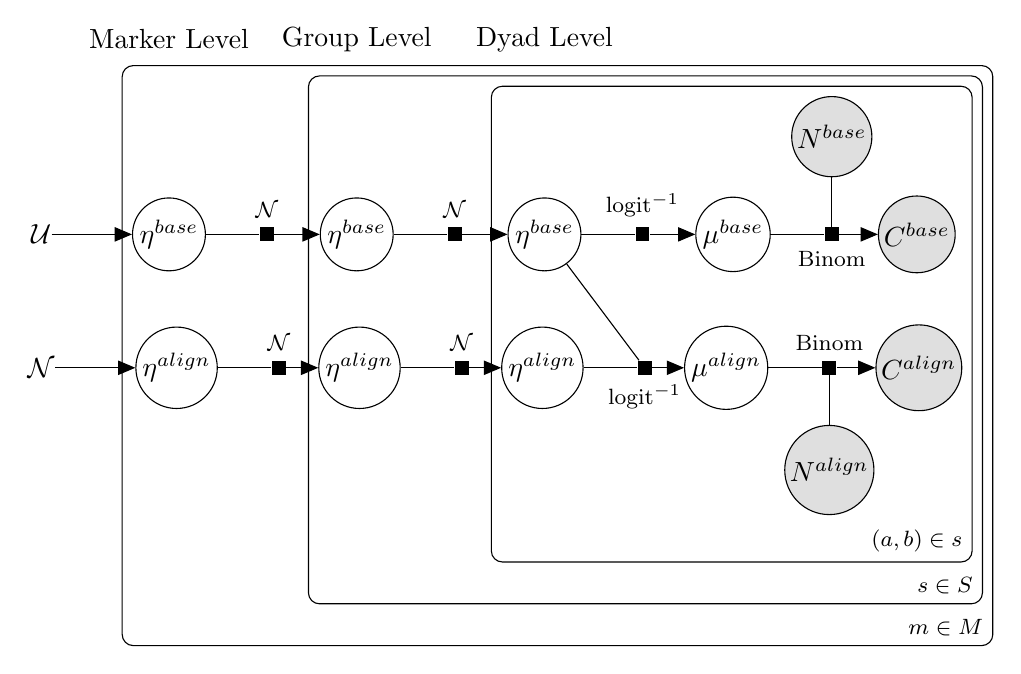
\begin{tikzpicture}[x=1.7cm,y=1.8cm]

  % Nodes

  \node[const] (base) {$\mathcal{U}$};
%  \node[latent,right=.6 of base] (n_b_m) {$\eta^{base}_m$}; 
%  \node[latent,right=.8 of n_b_m] (n_b_ms) {$\eta^{base}_{m,s}$};
%  \node[latent,right=.8 of n_b_ms] (n_b_mab) {$\eta^{base}_{m,a,b}$};
%  \node[latent,right=.8 of n_b_mab] (m_b_mab) {$\mu^{base}_{m,a,b}$};
%  \node[obs,right=.8 of m_b_mab] (C_b_mab) {$C^{base}_{m,a,b}$};

  \node[const,below=.8 of base] (align) {$\mathcal{N}$};
% \node[latent,right=.6 of align] (n_a_m) {$\eta^{align}_m$}; 
% \node[latent,right=.75 of n_a_m] (n_a_ms) {$\eta^{align}_{m,s}$};
% \node[latent,right=.75 of n_a_ms] (n_a_mab) {$\eta^{align}_{m,a,b}$};
% \node[latent,right=.75 of n_a_mab] (m_a_mab) {$\mu^{align}_{m,a,b}$};
% \node[obs,right=.8 of m_a_mab] (C_a_mab) {$C^{align}_{m,a,b}$};

  \node[latent,right=.6 of base] (n_b_m) {$\eta^{base}$}; 
  \node[latent,right=.85 of n_b_m] (n_b_ms) {$\eta^{base}$};
  \node[latent,right=.85 of n_b_ms] (n_b_mab) {$\eta^{base}$};
  \node[latent,right=.85 of n_b_mab] (m_b_mab) {$\mu^{base}$};
  \node[obs,right=.8 of m_b_mab] (C_b_mab) {$C^{base}$};

  \node[latent,right=.6 of align] (n_a_m) {$\eta^{align}$}; 
  \node[latent,right=.75 of n_a_m] (n_a_ms) {$\eta^{align}$};
  \node[latent,right=.75 of n_a_ms] (n_a_mab) {$\eta^{align}$};
  \node[latent,right=.75 of n_a_mab] (m_a_mab) {$\mu^{align}$};
  \node[obs,right=.8 of m_a_mab] (C_a_mab) {$C^{align}$};

  
  \node[const,above=1.05 of n_b_m] (marker) {Marker Level};
  \node[const,above=1.02 of n_b_ms] (group) {Group Level};
  \node[const,above=1.02 of n_b_mab] (dyad) {Dyad Level};

  % Factors
  
  \factor[right=of n_b_m] {n_b_m_f} {above:$\mathcal{N}$} {} {};
  \factor[right=of n_b_ms] {n_b_ms_f} {above:$\mathcal{N}$} {} {};
  \factor[right=of n_b_mab] {n_b_mab_f} {above:$\textrm{logit}^{-1}$} {} {};
  \factor[right=of m_b_mab] {m_b_mab_f} {below:Binom} {} {};

  \factor[right=of n_a_m] {n_a_m_f} {above:$\mathcal{N}$} {} {};
  \factor[right=of n_a_ms] {n_a_ms_f} {above:$\mathcal{N}$} {} {};
  \factor[right=of n_a_mab] {n_a_mab_f} {below:$\textrm{logit}^{-1}$} {} {};
  \factor[right=of m_a_mab] {m_a_mab_f} {above:Binom} {} {};

  %\factor[right=of C_b_mab] {C_b_mab_f} {above:Binom$} {} {};
  
  %\factor[above=of X]     {X-f}     {Multi} {} {} ; %
  %\factor[above=of T]     {T-f}     {left:Multi} {} {} ; %
  %\factor[above=of theta] {theta-f} {left:Dir} {} {} ; %

  % More nodes
  %\node[latent, right=of X-f] (phi)  {$\phi$}; %
  %\node[const, above=of phi]  (aphi) {$\alpha_\phi$}; %

  %\factor[above=of phi] {phi-f} {right:Dir} {} {} ; %

%  \node[obs,above=.35 of m_b_mab_f] (N_b_mab) {$N^{base}_{m,a,b}$};
%  \node[obs,below=.35 of m_a_mab_f] (N_a_mab) {$N^{align}_{m,a,b}$};

  \node[obs,above=.35 of m_b_mab_f] (N_b_mab) {$N^{base}$};
  \node[obs,below=.35 of m_a_mab_f] (N_a_mab) {$N^{align}$};


  \edge{base}{n_b_m};
  \factoredge {n_b_m}  {n_b_m_f}     {n_b_ms} ; %
  \factoredge {n_b_ms}  {n_b_ms_f}     {n_b_mab} ; %
  \factoredge {n_b_mab}  {n_b_mab_f}     {m_b_mab} ; %
  \factoredge {m_b_mab,N_b_mab} {m_b_mab_f} {C_b_mab}; %
 
   \edge{align}{n_a_m};
  \factoredge {n_a_m}  {n_a_m_f}     {n_a_ms} ; %
  \factoredge {n_a_ms}  {n_a_ms_f}     {n_a_mab} ; %
  \factoredge {n_a_mab,n_b_mab}  {n_a_mab_f}     {m_a_mab} ; %
  \factoredge {m_a_mab,N_a_mab} {m_a_mab_f} {C_a_mab}; %
 %\factoredge {atheta} {theta-f} {theta} ; %
  %\factoredge {phi}    {X-f}     {X} ; %
  %\factoredge {aphi}   {phi-f}   {phi} ; %

  %\gate {X-gate} {(X-f)(X-f-caption)} {T}

  \plate {pairplate} { %
    (N_b_mab)(C_b_mab) %
    (m_b_mab)(n_b_mab) %
    (N_a_mab)(C_a_mab) %
    (m_a_mab)(n_a_mab) %
  } {$(a,b) \in s$}; %
  \plate {subpopplate} { %
    (pairplate) %
    (n_b_ms) (n_a_ms) %
  } {$s \in S$} ; %
  \plate {} { %
    (subpopplate) %
    (n_b_m) (n_a_m)
  } {$m \in M$} ; %

\end{tikzpicture}
%\endpgfgraphicnamed

%%% Local Variables: 
%%% mode: tex-pdf
%%% TeX-master: "example"
%%% End: 

  \end{center}
  \caption{The alignment-inference model. A chain of normal distributions generates a linear predictor $\eta$, which is converted into a probability $\mu$ for binomial draws of marker presence/absence.}\label{fig:model}
\end{figure*}

\subsection{Motivation}
Our primary goal in moving to a Bayesian model of alignment is to fulfill the desiderata that the DNM measure does not.  Specifically, we want to improve the measure's consistency across different marker frequencies and its robustness to sparse data.  

To improve on this first point, we change the form of our alignment estimate from an additive effect in probability space to an additive effect in log-odds space. Having alignment as an additive effect in probability space means that the range of possible alignment strengths moves with the baseline; a more frequent marker can not show as much convergence as a less frequent marker can.  For our measure, we will treat alignment as a linear effect in log-odds space; this defines the alignment effect on the range $(-\infty,+\infty)$ and theoretically frees it from the influence of baseline probability, since even high probabilities can increase by large amounts in log-odds space.

To improve on the second point, we introduce a hierarchical prior on alignment values by marker and dyad. In doing so, we introduce an assumption that, unless the data argues strongly otherwise, dyads are likely to have similar alignment behaviors on a given marker. This leads to more accurate estimates of marker frequency and alignment in sparse data dyads, since they are influenced by the dataset as a whole.  

%This hierarchical structure also separates the alignment value from the baseline frequency, combining them only to 


%The second problem for the DNM measure is its potential difficulties with sparse data. \cite{DNMEtAl2012} address this by limiting the dataset to pairs who exchange at least 10 messages, and use three aggregation methods to deal with the data loss. However, the use of a such a cutoff could change the data substantially; people who repeatedly exchange messages may treat each other differently from people who exchange a very small number. In many offline settings, this difference is less critical, as the datasets contain a relatively small number of people exchanging a relatively large number of messages.  However, in many online settings, a large number of users exchange a smaller number of messages with each other, and there may be a substantial divide in the interaction styles of a pair with few, often unsolicited messages, and friends exchanging a flood of messages.\footnote{Users who send unsolicited and often unfriendly or otherwise non-conversational messages are known as  as trolls, randos (from ``random''), or---specific to Twitter---eggs, after the default egg-shaped avatar of a new, anonymous user. [TODO: what's the right word for "non-conversational" here?]}

%To deal with sparser data, we infer marker probabilities based on a simple generative model framework.  We will discuss a particular implementation here but also explain how this framework can be expanded to alignment studies with different proposed structures. 

\subsection{Model structure}
We begin by conceptualizing a conversation as a tree; each message, aside from the first, is in response to a particular preceding message, but a message may elicit multiple replies. (Tweets explicitly include which tweet number a reply is directed to.)  
For linguistic alignment purposes, we will represent a conversation as a set of message pairs. Suppose we observe a conversation that starts with  Alice says ``hi''. Bob replies to this message with ``hello there'', and Alice responds with ``how are you?''. In addition, Eve jumps into the conversation by replying to Bob with ``hi Bob!''.  This defines three message pairs: $[(A: hi), (B: hello there)]; [(B: hello there), (A: how are you?)]; [(B: hello there), (E: hi Bob!)]$.  We will focus on alignment effects in these pairs.

Following \cite{DNMGamonDumais2011}, we treat messages as binary vectors over words, rather than probability distributions or counts over words.  Because these are conversational messages, they tend to be short -- in the particular case of Twitter, messages contain on average approximately 3 to 6 markers---and thus this binarization instead of a count is not a severe simplification.\footnote{In fact, the shortness of the messages could introduce substantial noise if converting to a probability distribution per tweet, reducing robustness to sparse data.}  Alignment in this framework is an increase in the probability of seeing a given marker (or marker category) in the second message of a pair given that it appeared in the first message of that pair.


We can then treat the presence of a marker in a given tweet as a Bernoulli draw, with a marker-specific and dyad-specific probability $\mu^{base}_{m,a,b}$. This represents the baseline probability of a marker $m$ for a reply by speaker $b$ to speaker $a$ in which $a$ did not use $m$.  When the preceding message does contain $m$, the reply is instead modeled as a Bernoulli draw with a separate marker- and dyad-specific probability $\mu^{align}_{m,a,b}$.

We generate these two $\mu$ values from a hierarchical Gaussian structure in log-odds space, shown in Figure \ref{fig:model}.  Starting with the baseline values, a marker-specific $\eta^{base}_m$ is drawn from a uniform distribution on the interval $[-5,5]$. This $\eta^{base}_m$ represents the mean over potential $\mu^{base}_{m,a,b}$ values, defined in log-odds space, akin to the coefficients in a logistic regression. This range translates to approximately $[.006,.993]$ in probability space.  While in principle $\eta^{base}_m$ should range over all the real numbers, allowing the markers to have any probability between $0$ and $1$, the markers we are considering in the present work are all known to have per-message frequencies in the interval $[0.1,0.6]$, and thus the limited distribution is appropriate.\footnote{\cite{GelmanEtAl2008} discuss the $[-5,5]$ interval for logistic regression coefficients as capturing likely coefficients; for modeling markers with very high or low probabilities, the Cauchy distribution recommended in that paper could replace the uniform distribution, allowing (rare) extreme $\eta^{base}_m$ values.}  

One of our major goals with this model is to investigate the effect of sociological variables on alignment. Thus the $\eta^{base}_m$ value is used to define the mean of a normal distribution $N(\eta^{base}_m,\sigma^2)$, which is used to generate a set ``sub-population'' values $\eta^{base}_{m,s}$.  The sub-populations are based on the sociological features of the speaker pairs; in our data, we will be assigning pairs into subpopulations based on the power differential between them.\footnote{In terms of the general framework, this layer may be omitted if the potential for sub-population differences is not being investigated, or expanded if the sociological features require a more complex structure.} The $\eta^{base}_{m,a,b}$ value for a conversation dyad $(a,b)$ is drawn from a Gaussian distribution $N(\eta^{base}_{m,s},\sigma^2)$, where $s$ is the sub-population that the dyad $(a,b)$ belongs to. This marker- and dyad-specific $\eta^{base}_{m,a,b}$ is inverse-logit-transformed into a probability $\mu^{base}_{m,a,b}$, which is used to determine the number of times $C^{base}_{m,a,b}$ that speaker $b$ uses $m$ in response to $a$, based on $U^{base}_{m,a,b}$ Bernoulli draws, the number of times that $a$ spoke to $b$ without using $m$.

The alignment value $\eta^{align}_m$ is drawn from a normal distribution $N(0,\sigma^2)$, and as with the $\eta^{base}$ parameters, passes through a hierarchy of normal distributions at the subpopulation and dyad levels. Our goal with this parameter is to directly estimate the additive effect of alignment in log-odds space, so the probability $\mu^{align}_{m,a,b}$ is calculated as the inverse-logit of $\eta^{base}_{m,a,b}+\eta^{align}_{m,a,b}$.  If $\eta^{align}_{m,a,b} = 0$, there is no alignment; positive values indicate convergence, negative values divergence.

\subsection{Model Fitting and Inference}
Alignment measures can be extracted from multiple different levels of this model hierarchy; we focus on the $\eta^{align}_{m,s}$ parameter, which is a single value estimating the mean alignment by dyads within a subpopulation.\footnote{For a replication of the DNM measure, $\mu^{align}_{m,a,b}-\mu^{base}_{m,a,b}$ could be calculated instead.}  This value represents the change in the log-odds of using $m$ when replying to someone who has already used it, our operationalization of alignment.

We implemented this model in RStan \cite{?}, with code available at \url{http://github.com/langcog/alignment}. We run the model over 200 iterations (100 of them discarded as burn-in) for each dataset.  Alignment estimates are extracted from each of the final 100 iterations of the model inference, and we use bootstrapping over these parameter estimates to set a 95\% confidence interval on the parameter values, which will be reported in each of the plots.

% We suppose that different speakers and repliers may have different baseline usages.\footnote{This is an important assumption, as work in authorship attribution has found consistent and distinctive by-person usage rates for many of the function words that we use as markers.\cite{?}} This can be implemented either at the level of individuals or at a subpopulation level, with the subpopulations defined by sociologically relevant features (in our test case, verification status on Twitter). These values are implemented in logit space so that they can be defined over $ [-\infty,+\infty] $ and converted to probabilities using the inverse logit function. These subpopulation usage values are in turn drawn independently for each marker, as different markers may have different baseline rates or different alignment rates.  Finally, means for each marker over the population as a whole are drawn from a normal distribution that serves primarily as a regularizer.  [TODO: probably swap order to start with hgihest-level draw and work down to individuals.]

%Our focus is on alignment, the change in a marker's probability when the preceding message has used that marker versus when it has not.  There are potentially many ways of calculating this change; we break from the subtrcative conditional probability measure and 

\section{Experiment 1: Simulations}
Our first experiment uses simulated data to assess the DNM measure and our new model-based approach on the quantitative desiderata: consistency across different marker frequencies, robustness to sparse data, and measure sensitivity.

\subsection{Simulation 1: Binary presence/absence}
Our first simulation treats the presence or absence of a marker as the relevant quantity. Instead of attempting to estimate word productions based on unigram probabilities and known message lengths, we simplify the process by generating messages with a given probability of containing the marker.  This more closely resembles the generative process in our model.

We again start by generating a set number dyads, in this case $500$, representing people who are observed talking to each other. For each dyad, we draw a number of messages exchanged from a geometric distribution with mean $5$. For each message, we decide perform a Bernoulli draw with probability $p(A)$ that the message will contain the marker.  (Conditionalized, baselined alignment can not be calculated unless the first member of the dyad has at least one message containing the marker and one message not containing the marker to estimate the effect on the replier. Dyads that do not meet the criterion are re-drawn.) If a message does not contain the marker, its reply contains the marker with the same probability $p(A)$. If the message does contain the marker, though, we increase the probability of the reply containing the marker by adding an alignment strength $\alpha$ in log-odds space, which keeps the probabilities inside the $[0,1]$ range. $\alpha = 0$ implies no alignment; positive $\alpha$ represents the standard linguistic convergence, negative $\alpha$ the rarer divergence \cite{Ferrara1991}.  We test over a range of marker baseline probabilities that cover the range of the marker frequencies in the Twitter data of the next section. 

Figure \ref{fig:sim1} shows the result of the DNM measure and our model-based measure.  (LSM and LLA are not evaluated in this simulation because they require by-word calculation; see Simulation 2.) DNM shows a rapidly decreasing slope as the marker baseline frequency increases.  Additionally, within a given baseline frequency, the relationship between true and estimated alignment is non-linear, especially at high or low marker frequencies.  Our model-based measure has a more linear relationship between true and estimated alignment, although it does display a slight ceiling effect with high marker frequency and high positive alignment.  In addition, the slope of the true-estimated alignment relationship is much more consistent across different marker frequencies.  These results show that our model satisfies the marker frequency consistency desideratum better than the DNM measure.

\begin{figure}[t]
\centering
\includegraphics[width=\columnwidth]{graphics/www2016_simulation1_crossiter.pdf}
\caption{Results from simulation 1. Plot shows the actual alignment values from the simulations against the model-inferred values of the alignment. Ranges shown are bootstrapped 95\% confidence intervals; lines are loess-fit curves. The DNM measure shows substantial influence of the marker's baseline probability; the model-inferred alignments are more consistent across a range of alignments.}\label{fig:sim1}
\end{figure}

\subsection{Simulation 2: By-word generation}
Our second simulation uses a slightly more complex generative process, first generating a length for a message and then filling in words within the message.  This moves closer to the true generative process underlying person-to-person conversation, and further from our model's binarized generative process.  It also allows us to test the LLA and LSM measures on simulated data. [TODO: add variance-by-data-size analysis/plot.]

We again start by generating $500$ interacting dyads, exchanging a number of messages drawn from a geometric distribution with mean 5. Each message has a number of words draw from a uniform distribution on the interval $[1,25]$, approximating the 140-character limit of Twitter. For a given marker, we specify a unigram probability $p(w)$ and generate all messages from the first member of the dyad based on this probability. (As above, dyads where the first user either always or never uses the marker are re-drawn.) If the initial message does not contain the marker, the reply is also generated with unigram probability $p(w)$. If the initial message does contain the marker, the reply marker unigram probability is increased by $\alpha$ in log-odds space.  We vary the marker frequencies over a range representative of common words ($.005 \approx by$, $.01 \approx that$, $.05 \approx the$ in \cite{Brown}) or word categories ($.1 \approx $ personal pronouns, $.2 \approx $ all pronouns, in \cite{KacewiczEtAl2013}), appropriate comparisons for the marker categories used in the Twitter experiments of the next section.

Figure \ref{fig:sim2} shows the relationship between true and estimated alignments over different marker frequencies.As in the earlier simulations, the DNM measure is positively correlated with true alignment, but the relationship is somewhat non-linear and dependent on the marker frequency.  The model-based estimates again outperform the DNM measure, with consistent estimates across a wider range of marker frequencies.  With conditionality but no baselining, discriminate LLA is able to detect changes in the (positive) alignment strength, but is greatly affected by a marker's baseline frequency.  LSM fails in this simulation to correctly capture alignment, estimating the greatest ``alignment'' when there is no simulated alignment.  This is because  the speakers in this simulated dataset all have the same baseline marker frequencies; thus, if they speak independently of each other, their rate of marker usage will be approximately the same. If the replier conditions their marker use on the initial speaker, the replier's rate of marker usage will move away from that of the speaker, reducing LSM.  This shows that LSM actually quantifies the homophily of a dyad, rather than their alignment.

\begin{figure}[t]
\centering
\includegraphics[width=\columnwidth]{graphics/www2016_simulation2b_crossiter.pdf}
\caption{Results from simulation 2. Plot shows the actual alignment values from the simulations against the model-inferred values of the alignment. Ranges shown are bootstrapped 95\% confidence intervals over different simulation runs; lines are loess-fit curves.}\label{fig:sim2}
\end{figure}

On the whole, these simulations provide evidence that the conditionality/baseline desideratum is critical for separating out alignment from homophily.  We also find that the model-based measure is better at satisfying the marker frequency consistency desideratum than any of the other tested measures.


%\begin{figure*}
%\centering
%\includegraphics[width=.9\textwidth]{graphics/www2016_simulation2_simple.pdf}\label{fig:sim2}
%\caption{Results from simulation 2. Rows are different alignment measures; columns different baseline word frequencies.  Ranges shown are bootstrapped 95\% confidence intervals over different simulation runs. Opaque parameters indicate false positives or false negatives.}
%\end{figure*}


\section{Experiment 2: Twitter and Power}
With the simulation results in hand, we turn to an examination of alignment on Twitter.  Alignment on Twitter was initially investigated by \cite{DNMGamonDumais2011}, who found overall positive alignment on all 14 marker categories, but no significant effects of social power/status on alignment, contrary to findings of power/status effects in many other settings \cite{Gnisci2005}, including some Web-based settings \cite{DNMEtAl2012,NobleFernandez2015}.  It is possible that social media does not display power/status-based differences in alignment, perhaps because status differences are less obvious in the social media setting, but it is also possible that the differences are subtler or situated in a more noisy environment than in other settings, and that the improved resolution of the model-based measure can detect them.  This experiment presents evidence of the latter possibility, that power differentials do affect alignment on social media.

\subsection{Corpus}
We use a collection of Twitter conversations collected by \cite{DoyleFrank2015CMCL} to examine information density in conversation. This corpus focuses on conversations within a set of 14 mostly distinct subcommunities on Twitter.  These subcommunities contain all the messages exchanged between Twitter users who sent at least one message to a ``seed user'' with a reasonably large number of followers. This corpus contains 63,673 conversation threads, covering 228,923 total tweets.  We divide these conversations into message pairs, also called conversational turns, which are two consecutive tweets within a conversation thread.  The second tweet is always an explicit reply to the first, and the two tweeters in the pair must be distinct.  

One additional piece of processing is done; while formal retweets (sharing another tweeter's message to one's own timeline) are removed from the data automatically, there are a variety of informal retweeting methods that are not marked by the Twitter API.  We therefore removed all pairs where the reply tweet contained all of the words of its preceding tweet and additionally had either the bigram \textit{RT @username:} (indicative of a ``manual retweet'') or Unicode curly quote characters (indicative of a type of quoting that some Twitter apps use).  In these cases, the entirety of the previous message was included, ensuring maximal alignment, but the words were provided as repetition of a quote rather than being produced as part of the replier's message.  This leaves us with [TODO: count] message pairs, spanning [TODO: count] users.

The tweets were parsed into word tokens using Twokenizer \cite{OwoputiEtAl2013}, with usernames and URLs removed.  We then calculated linguistic alignment on the fourteen marker categories used by \cite{DNMGamonDumais2011} in their study of Twitter messages.  These categories come from the Linguistic Inquiry and Word Count (LIWC) system \cite{LIWC}; category names and sample words are shown in Table \ref{tab:LIWC}. These categories were chosen (from the complete set of 74 [TODO: check] LIWC categories) as ``strictly non-topical style dimensions'' as they had limited to no content words in them, and were not focused on specific topics.  These can be roughly divided into four pronoun categories (indefinite, 1st singular, 1st plural, 2nd), four other syntactic categories (article, conjunction, preposition, quantifier), and six conceptual categories (certainty, discrepancy, exclusive, inclusive, negation, tentative).

A tweet is counted as containing a given category if it contains at least one word from that category.  Alignment is calculated based on category rather than on specific word types; thus if the first tweet contains \textit{an} and its reply contains \textit{the}, this counts as an example of positive alignment.

\begin{table}
\centering
\caption{Marker categories for linguistic alignment, with examples, number of distinct types, and probability of appearing in a tweet.}\label{tab:LIWC}
\begin{tabular}{|c|c|c|c|} \hline
Category & Examples & Size & $p(A)$\\ \hline
Article & \textit{a, an, the} & 3 & .44 \\
Certainty  & \textit{always, never} & 83 & .18 \\
Conjunction  & \textit{but, and, though} & 28 & .39\\
Discrepancy  & \textit{should, would} & 76 & .20 \\
Exclusive  & \textit{without, exclude} & 17 & .27\\
Inclusive  & \textit{with, include} & 18 & .30\\
Indefinite pronoun  & \textit{it, those} & 46 & .39\\
Negation  & \textit{not, never} & 57 & .21\\
Preposition  & \textit{to, in, by, from} & 60 & .58\\
Quantifier  & \textit{few, many} & 89 & .26\\
Tentative & \textit{maybe, perhaps} & 155 & .23\\
1st person singular  & \textit{I, me, mine} & 12 & .57\\
1st person plural & \textit{we, us, ours} & 12 & .14\\
2nd person pronoun   & \textit{you, yourself} & 20 & .25\\
\hline\end{tabular}
\end{table}

\subsection{Overall Alignment}
\cite{DNMGamonDumais2011} found significant positive alignment on all fourteen marker categories on Twitter, but did not detect an effect of power on alignment.  We start by replicating the overall positive alignment result before moving on to the effects of power.  Figure \ref{fig:overall-alignment} shows the alignment values for this Twitter dataset using the measure from \cite{DNMGamonDumais2011} on the left, and our model-based alignment measure on the right.  95\% confidence intervals are shown, based on 1000-draw bootstrapping. [TODO: fix description of error bars] As expected, both measures find consistent and significant convergent alignment on all fourteen marker categories.  

\begin{figure}[t]
\centering
\includegraphics[width=.9\columnwidth]{graphics/www2016_alignmentdnmour_uniform.pdf}
\caption{Overall alignment per marker category for DNM-style and model-based alignment. All 14 marker categories show significant convergent alignment. [TODO: fix axes -- ggplot is being a real pain] [TODO: sort the markers into categories]}\label{fig:overall-alignment}
\end{figure}


\subsection{Alignment and Power}
We are especially interested in applying the model-based measure to the specific question of whether power influences the strength of alignment, as has been shown in other settings \cite{DNMEtAl2012,NobleFernandez2015}. Previous work \cite{DNMGamonDumais2011} showed that Twitter users do align to each other on average, but did not show increased alignment to power.  We expect that the improved sensitivity of our model-based alignment measure will show the anticipated effect of alignment to power.

We assess power on Twitter in two ways. First, we use twitter user verification as an external measure of power.  Twitter verifies important people to show that their account is really them, and not a name squatter, impostor, or parody account.  Verified accounts range from heads of state (\texttt{@POTUS, @MedvedevRussiaE}) to famous athletes (\texttt{@KingJames,@Shaq}) to Youtube stars (\texttt{@camerondallas,@pewdiepie}).  These represent people who Twitter considers significant, generally for accomplishments outside of social media.  Second, we use follower counts to assess power internal to the Twitter network.  Users with more followers have their tweets read by more users, get more retweets and favorites, and so on, lending them power within the network.  In addition, if they retweet or reply to another user, it can substantially increase that user's status and follower count.  As such, we expect that both verified users and users with high follower counts will be aligned to more than unverified users and users with small follower counts.

Intuitively, this is the idea that we show deference to important tweeters that we do not show to our friends. While such increased alignment to powerful people has been observed in many non-Web settings \cite{?}, it is possible that the different dynamics of social media would remove or even reverse this effect.  Trolls, cranks, and a variety of other non-cooperative conversationalists may fill people's Twitter timelines, and some celebrities and athletes have left or avoided Twitter for this reason \cite{?}.  However, we predict that social media is not so different from other settings, and that a sufficiently sensitive measure may find an effect of power.

\paragraph{Verification as power} For power in terms of verification, we look specifically at tweet pairs where the replier is unverified.  Because there are relatively few verified users, there were few verified reply tweets in our dataset, and especially few tweets from verified users to other verified users. We focus instead on how unverified, average-Joe repliers adjust their alignment depending on the verification status of the original tweet's sender.  We predict that tweets sent from an unverified user to a verified user will show greater alignment than tweets sent from an unverified user to a fellow unverified user.  

\begin{figure}[t]
\centering
\includegraphics[width=.9\columnwidth]{graphics/www2016_dnmpowerdiff_verif.pdf}
\caption{Difference in DNM-style alignment on the 14 marker categories when speaking to verified or unverified users. Positive values indicate greater alignment to verified users; negative indicates greater alignment to unverified users. No markers show significant effects of power on alignment.}\label{fig:dnm-verified}
\end{figure}

Figure \ref{fig:dnm-verified} shows the mean difference in per-category alignments when unverified users reply to verified versus unverified users, according to the DNM measure.  A positive value indicates increased alignment to the verified, powerful tweeters.  However, none of the marker categories show significant increases in alignment to verified users, based on the 95\% confidence intervals from a 1000-sample bootstrap.  This replicates the result in \cite{DNMGamonDumais2011}, using their measure.

Figure \ref{fig:our-verified} shows the difference between alignment to verified and unverified tweeters according to the model-based measure. Here we see positive differences, indicating higher alignment to verified tweeters, on more than half of the categories.  The one category that shows a negative difference is the second person pronoun category (e.g, \textit{you, yourself, y'all}), which is not entirely unexpected. Work on power dynamics in language have shown that many personal pronouns are used differently by those with and without power \cite{KacewiczEtAl2013,ChungPennebaker2007}, and as such there may be differences in whether \textit{you}-usage triggers reciprocation between two unverified users, of similar social standing, versus between a powerful and non-powerful person.

\paragraph{Follower ratios as power} Our second measure of power is based on users' relative numbers of followers.  Unlike verification, this is an intrinsic measure of power, reflecting one's importance within Twitter -- although verified users generally also have more followers than unverified users do. For each pair of users, we calculate their \textit{follower ratio} by dividing the first tweeter's follower count by the sum of their follower count and their replier's follower count.  Numbers above 0.5 indicate that the first tweeter has more followers than the replier.  We take 0.99 as our cutoff, meaning that the first tweeter has at least 99 times as many followers as the replier.  [TODO: calculate percentage] of our pairs have this property.  Under the hypothesis of increased alignment to power, we expect to find increased alignment when the follower ratio is above 0.99. [TODO: note that we do not separately look at low speaker follower count ratios, because high follower count people very rarely talk enough to low follower count people to assess alignment.]

\begin{figure}[t]
\centering
\includegraphics[width=.9\columnwidth]{graphics/www2016_dnmpowerdiff_fratio.pdf}
\caption{Difference in DNM-style alignment on the 14 marker categories depending on follower ratio. Positive values indicate greater alignment to high-follower users; negative indicates greater alignment to low- and equal-follower users. One category, first-person plural pronouns, shows a significant \textit{negative} effect of power on alignment, while the rest show no effect.}\label{fig:dnm-fratio}
\end{figure}

Figure \ref{fig:dnm-fratio} shows the difference in alignment to power derived from follower counts, using the DNM measure. Here one category has a significant effect of power on alignment -- first-person plurals, which, like the second-person pronouns in the verification-power experiments, may have different usage patterns for those with and without power.  The rest of the categories show no significant effects.  Again, this appears to replicate the lack of significant alignment to power found by \cite{DNMGamonDumais2011}.

Figure \ref{fig:our-fratio} shows the alignment differences based on power derived from follower counts, using our model-based measure.  As with the verification-based power, we see significantly more alignment to powerful users in most categories. First-person plural pronouns are an outlier by this measure, as they were according to the DNM measure.  Overall, though, we see significantly higher alignment to power.

\begin{figure}[t]
\centering
\includegraphics[width=.9\columnwidth]{graphics/www2016_ourpowerdiff_fratio.pdf}
\caption{Difference in model-based alignment on the 14 marker categories depending on follower ratio. Ten markers show significantly more alignment to power; three of the four that do not are pronouns.}\label{fig:our-fratio}
\end{figure}

  Crucially, we see substantial evidence for a general increase in alignment to a user with more social power, even if that social power is extrinsic to the social network.

Interestingly, we see compelling evidence for the non-monolithic nature of linguistic alignment. All of the marker categories showed an overall positive alignment effect (Figure \ref{fig:overall-alignment}), but when we compare differences in how people align to with or without power, the markers show idiosyncratic effects.  One class of markers, the pronouns, have previously been shown to interact with power \cite{KacewiczEtAl2013}, and these consistently show less alignment to power than most other markers. Detecting such patterns is a key reason behind the marker separability desideratum.

\begin{figure}[t]
\centering
\includegraphics[width=.9\columnwidth]{graphics/www2016_ourpowerdiff_verif.pdf}
\caption{Difference in model-based alignment on the 14 marker categories when speaking to verified or unverified users. Positive values indicate greater alignment to verified users; negative indicates greater alignment to unverified users. Seven markers show significantly more alignment to power; only five show significantly less.}\label{fig:our-verified}
\end{figure}

\section{Conclusions}
Accommodation to one's conversational partners is a deeply ingrained human characteristic, important for assessing the nature of conversation.  Standardized and formalized measures of this accommodation, especially in terms of linguistic alignment, have been lacking, and this has limited analysis of accommodation, especially in non-traditional settings, such as social media.  We proposed a set of five desiderata for a measure of linguistic alignment: conditionality/baselining, marker separability, consistency across marker frequencies, robustness to sparse data, and sensitivity.  We designed a model-based framework for assessing alignment in Twitter conversations, and showed that this framework is able to detect differential alignment based on differences in social status that were undetectable by previous measures.  This framework can be extended and applied to other Web-based and face-to-face conversational settings as well.

%\end{document}  % This is where a 'short' article might terminate

%ACKNOWLEDGMENTS are optional
%\section{Acknowledgments}


%
% The following two commands are all you need in the
% initial runs of your .tex file to
% produce the bibliography for the citations in your paper.
\clearpage
\bibliographystyle{abbrv}
\bibliography{library}  % sigproc.bib is the name of the Bibliography in this case
% You must have a proper ".bib" file
%  and remember to run:
% latex bibtex latex latex
% to resolve all references
%
% ACM needs 'a single self-contained file'!
%
%APPENDICES are optional
\balancecolumns

\end{document}
